
        \documentclass{exam-zh}
        \usepackage{siunitx}
        \examsetup{
          page/size=a4paper,
          paren/show-paren=true,
          paren/show-answer=false,
          fillin/show-answer=false,
          solution/show-solution=false
        }
        \ExamPrintAnswerSet{
          sealline/show=true,
          page/size=a3paper,
          paren/show-answer=false,
          fillin/show-answer=false,
          solution/show-solution=false,
        }
        \everymath{\displaystyle}
        \title{赵一涵 四年级下学期练习}\subject{四则混合运算}\begin{document}\maketitle\begin{question}猪能上树\paren\end{question}\begin{question}$1+1=$\paren\begin{choices}\item $1$\item $2$\item $3$\end{choices}\end{question}\begin{question}猪一般是上\fillin[]的树\newline 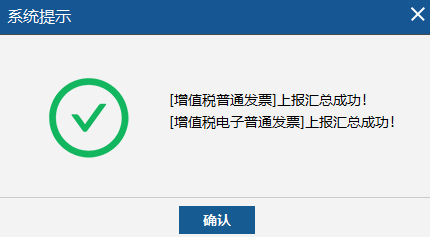
\includegraphics[width=5cm]{test.png}\end{question}\begin{question}已知$2x$是$216$的立方根,则$x+6$的平方根是\underline{\hspace{1cm}}\end{question}\end{document} 